% VLDB template version of 2020-08-03 enhances the ACM template, version 1.7.0:
% https://www.acm.org/publications/proceedings-template
% The ACM Latex guide provides further information about the ACM template

\documentclass[sigconf, nonacm]{acmart}
\usepackage{caption}
\usepackage{subcaption}
%% The following content must be adapted for the final version
% paper-specific
\newcommand\vldbdoi{XX.XX/XXX.XX}
\newcommand\vldbpages{XXX-XXX}
% issue-specific
\newcommand\vldbvolume{14}
\newcommand\vldbissue{1}
\newcommand\vldbyear{2020}
% should be fine as it is
\newcommand\vldbauthors{\authors}
\newcommand\vldbtitle{\shorttitle} 
% leave empty if no availability url should be set
\newcommand\vldbavailabilityurl{https://github.com/Lennart97/nlp_project}
% whether page numbers should be shown or not, use 'plain' for review versions, 'empty' for camera ready
\newcommand\vldbpagestyle{empty} 
\settopmatter{printfolios=true}

\begin{document}
\title{Predicting political views based on tweets}

%%
%% The "author" command and its associated commands are used to define the authors and their affiliations.
\author{Florian Siepe}
\affiliation{%
  \institution{Philipps University of Marburg}
  \city{Marburg}
  \state{Germany}
}
\email{Siepe@students.uni-marburg.de}

\author{Lennart Hallenberger}
\affiliation{%
	\institution{Philipps University of Marburg}
	\city{Marburg}
	\state{Germany}
}
\email{Hallenb@students.uni-marburg.de}

%%
%% The abstract is a short summary of the work to be presented in the
%% article.
\begin{abstract}
In this work, we discuss and evaluated a topic modeling approach towards predicting political views of users based on their tweets. 
A dataset was used, which contains tweets of U.S. American politicians from the Democratic and Republican Party. 

After cleaning and preprocessing the tweets, they are embedded using Latent Dirichlet Allocation (LDA) based on the topics they contain. 
With these embeddings, classifiers are trained to predict a political party based on a tweet. 
The results show that no reliably predictions can be made with this embedding technique.
\end{abstract}

\maketitle

%%% do not modify the following VLDB block %%
%%% VLDB block start %%%
\ifdefempty{\vldbavailabilityurl}{}{
\vspace{.3cm}
\begingroup\small\noindent\raggedright\textbf{PVLDB Artifact Availability:}\\
The source code, data, and/or other artifacts have been made available at \url{\vldbavailabilityurl}.
\endgroup
}
%%% VLDB block end %%%

\section{Introduction}
\label{sec:intro}
Over the past years, social media has become more relevant in politics. 
Not only are politicians them self’s using social media to gain a growing following, it’s also where citizens discuss and share their opinion on political topics.
From this comes an interest to classify social media posts by their political point of view. 
One use case can be to gain insights on political topics and their distribution amongst voters. Furthermore, analyzing posts in a large scale can play a role in more accurate projections of future elections.

The goal of this project is to classify users based on their social media postings regarding their political viewpoint to match them with a political party. 
To test the accuracy of our approach, we use tweets made by members of the Democratic and Republican Party from the United States (\ref{sec:data}).
Next we apply an LDA and train a classifier on these tweets to predict the party based on the tweets content (\ref{sec:app}). The results from the classifier are then evaluated and discussed (\ref{sec:eval}). Finally, we give a summary and point out the key findings (\ref{sec:summ}).

\section{Dataset}
\label{sec:data}
The used dataset \footnote{\url{https://www.kaggle.com/datasets/kapastor/democratvsrepublicantweets}} consists of 84502 tweets from May 2018. 
These tweets were collected from 433 accounts, whose author are validated members of either the Democratic or Republican Party. 
The tweets have an equal distribution with 49\% being written by Democrats and the remaining 51\% by Republicans.

For each account, the last 200 tweets were collected and labeled with their political party.

\section{Approach}
\label{sec:app}
The approach we use to predict the proximity to a political party consists of four main steps.

\begin{enumerate}
	\item Data cleaning
	\item Preprocessing
	\item Creating an LDA
	\item Classifier training and prediction
\end{enumerate}

\begin{figure}[h]
	\centering
	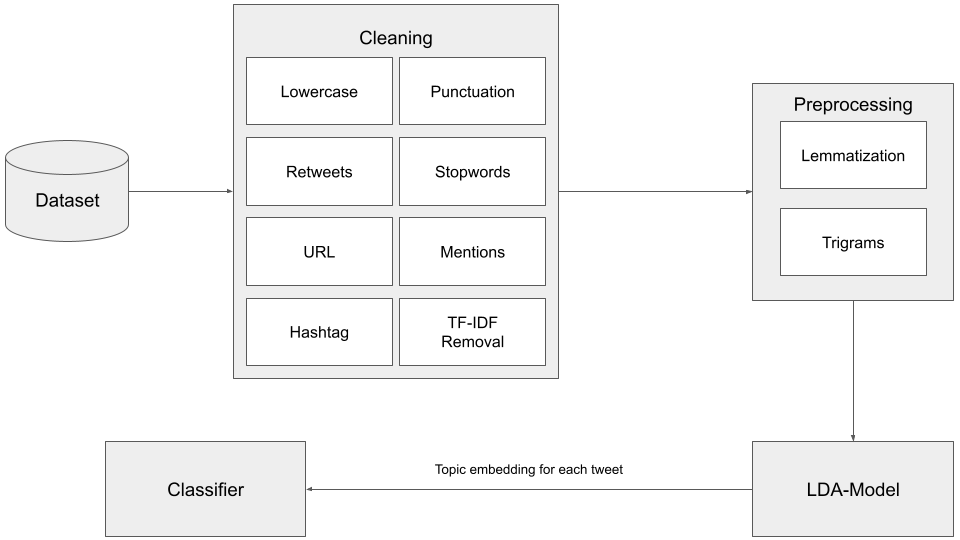
\includegraphics[width=0.9\linewidth]{figures/pipeline}
	\caption{Pipeline of the given approach}
	\label{fig:pipeline}
\end{figure}

Figure \ref{fig:pipeline} illustrates this process. In the following, each of the shown steps will be outlined in greater detail.

\subsection{Data cleaning}
\label{subsec:clean}
As tweets are usually noisy in terms of being grammatically correct and often contain human errors like typos, cleaning data from this noise is an essential step.

The cleaning is organized in different modules, each responsible to deal with a certain aspect of the data.

\paragraph{Lowercase} To avoid unnecessary ambiguity, all tokens are converted to lowercase.

\paragraph{Punctuation} Special punctuation characters are removed, as they do not carry semantic meaning.

\paragraph{Stop words} Similarly, stop words like "a" or "the" do not carry semantic meaning either, thus removing them as well.

\paragraph{Retweets} Retweets are a special feature of tweets such that a user repeats a tweet from a different user. However, since it can usually be assumed that retweeting means confirmation with the original tweets, only the respective marker is removed.

\paragraph{URL} Users often provide links to external resources in their tweets. Since extracting topics from these resources is out of scope of this project, URLs are removed from tweets.

\paragraph{Mentions} Twitter users can mention other users. For further improvements this information might be included to strengthen or weaken an existing classification based on the user's political view.

\paragraph{Hashtag} Hashtags express the tweets relevancy for a specific topic. Since users of both party's tweet about the same topics with opposing opinions hashtags appear as noise, thus being removed.

\paragraph{TF-IDF} Some tokens (or words) appear only a few times, while others occur quite often. Either way, this commonly means that these tokens are too specific and might lead to noise in the data, or they do not carry much meaning. Therefore, they might be removed.

\subsection{Preprocessing}
\label{subsec:process}
Having cleaned some aspects of the data, preprocessing is the next step. For this we utilize lemmatization and the creation of trigrams.

\paragraph{Lemmatization} To further reduce ambiguity and complexity of the data all words are being lemmatized and reduced to their base form.
While being computationally more expensive, this usually gives better results than stemming, which uses heuristics.

\paragraph{Trigrams} When analyzing word sequences and their meaning the order of words is an important aspect to be considered. To take this into account, we create trigrams to feed them into our model.

\subsection{Creating an LDA}
\label{subsec:lda}
Coming back to the main task, to distinguish political views, the essential part is finding features to differentiate between democrat and republican tweets. The difference must be representable in an embedding to train a classifier later for doing the actual classification. The key question is, how to find a unique word or word sequences which are specific for Democrats or Republicans.

In the following, we are outlining an approach using topic modeling. We use the commonly known LDA, a generative probabilistic model \cite{lda}.

In topic modeling, words (here trigrams) are collected in documents (tweets), where each word's presence is an indicator for a specific topic in the document. On the other hand, each topic also has various words belonging to it. Therefore LDA tries to find topics a document belongs to based on the word in the document.

While LDA is an unsupervised learning method, the number of desired topics $k$ needs to be specified upfront. 
Thus, another challenge is to find a $k$ where the distance between topics which are assigned to Democrats and Republicans is maximized. 
Section \ref{sec:eval} further explains how an optimal $k$ is found.

\subsection{Training a classifier}
\label{subsec:classify}
After creating a topic model on our data, the next step is training a classifier.

Clearly, an embedding has to be created upfront for our tweet dataset.
For this, we utilize the LDA we created before.
For each tweet the LDA is applied, which outputs a likelihood distribution over the topics, that indicates the likelihood for a tweet to contain specific topics.
The output of the LDA is a vector $\vec{v}$ with $|\vec{v}|=k$.

With this embedding, a classifier is trained against the respective labels "Democrat" and "Republican". To see how different classifier perform, we evaluate \textit{Gaussian Naive Bayes (G-NB)}, \textit{Linear Support Vector Machine (L-SVM)} and \textit{Multi-Layer Perceptron (MLP)}.

\section{Evaluation}
\label{sec:eval}
\begin{figure}[ht]
	\centering
	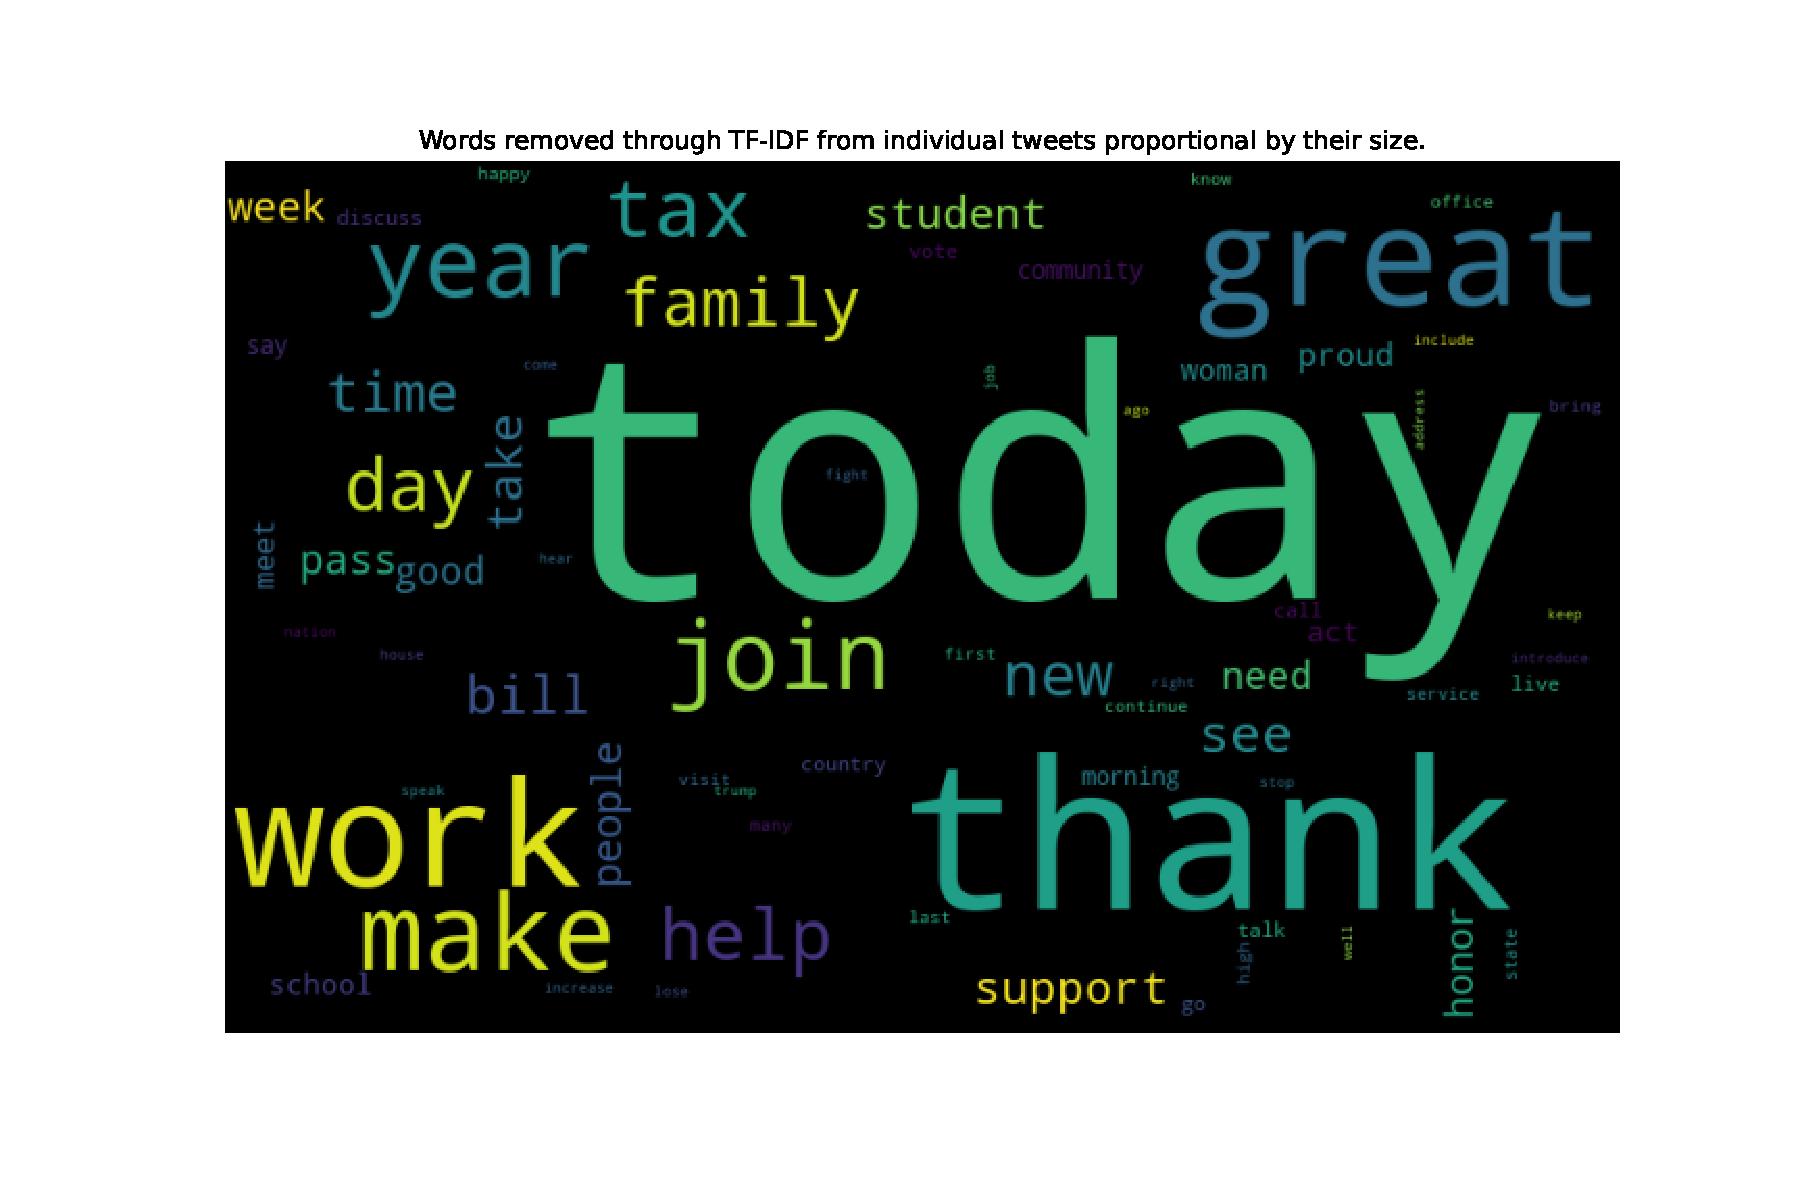
\includegraphics[width=0.95\linewidth, trim={3.5cm 3cm 3.5cm 2.7cm}, clip]{figures/40k/diff_wordcloud_tfidf.pdf}
	\caption{Words removed by TF-IDF}
	\label{fig:tfidf}
\end{figure}

Figure \ref{fig:tfidf} shows the words removed using TF-IDF during the data cleaning. The size of a word represents how often it was removed from tweets overall. Especially the biggest words shown, like "today", "thank" and "work" were often present in tweets by Democratic or Republican Party members. Removing these words resulted in a higher differentiation between topics by the LDA because of less overlapping words.

As outlined in \ref{subsec:lda} a topic count $k$ needs to be found. Therefore we created models with an increasing number of topics and measure the associated logarithmic perplexity and coherence (UMass) of the models.

\begin{figure}[h]
	\centering
	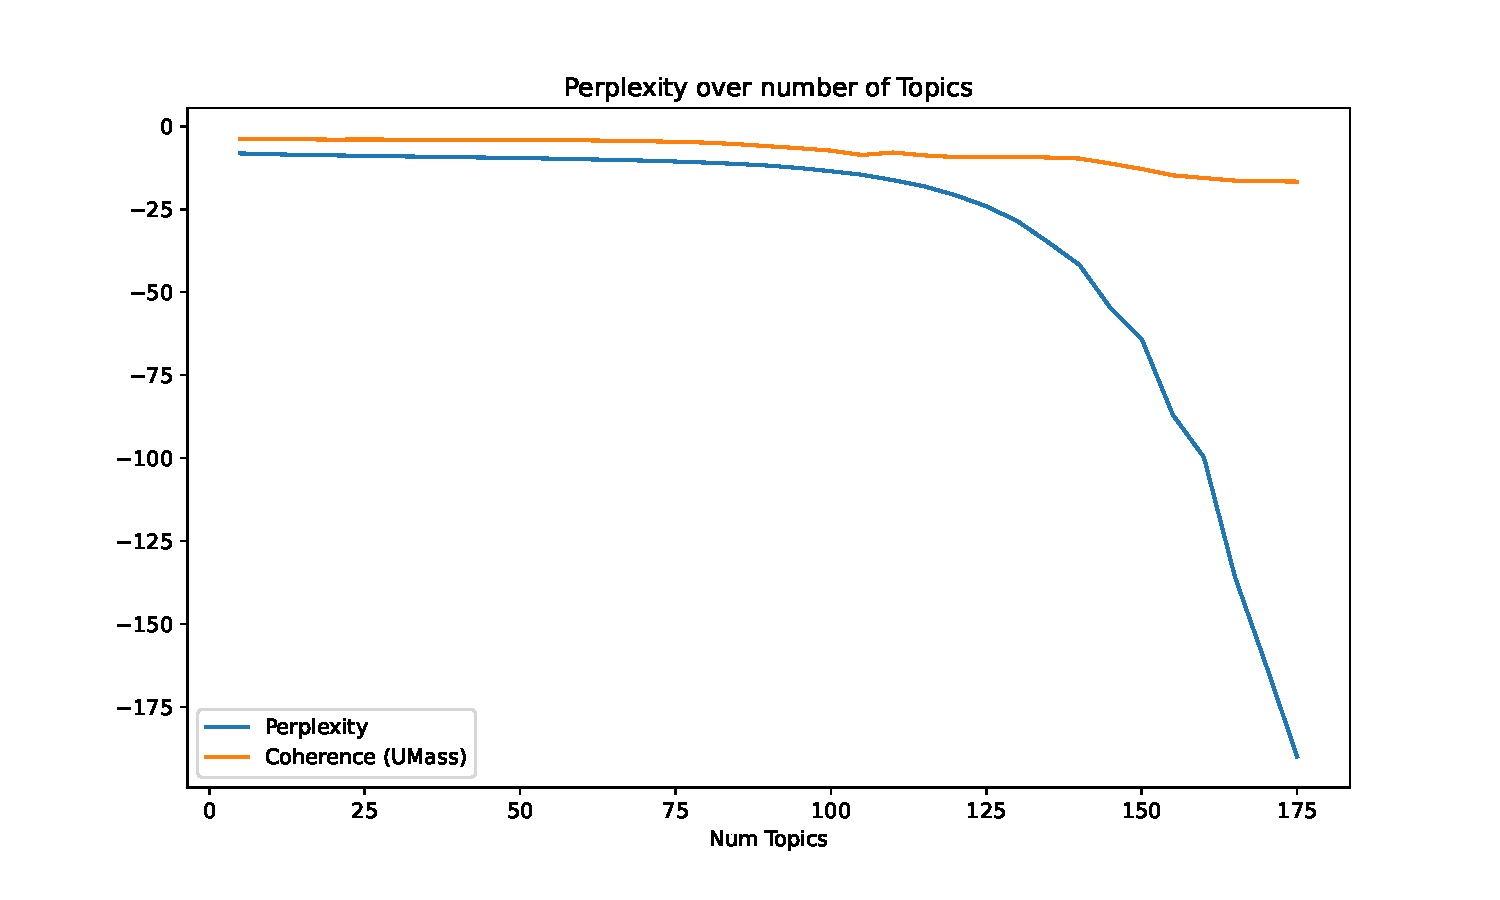
\includegraphics[width=\linewidth, trim={2cm 0cm 2cm 1.7cm}, clip]{figures/40k/perplexity_coherence_over_topics.pdf}
	\caption{logarithmic perplexity and coherence over $k$}
	\label{fig:topiccount}
\end{figure}

Figure \ref{fig:topiccount} shows the perplexity and coherence over $k$. Measurements of both values were collected starting with $k=5$ increasing the number of topics by 5 till $k=175$. We can observe a decline in perplexity and coherence with an increasing number of topics. While we see a slow but steady decline from the start, the perplexity drops significantly with $k>120$.

\newpage

Similarly, the performance of MLP, G-NB and L-SVM have been observed over the range of topics from $k=5$ to $k=175$ in steps of 5. 
With the results we can determine the optimal number of topics $k$ and the best performing classifier.


\begin{figure}[h]
	\centering
	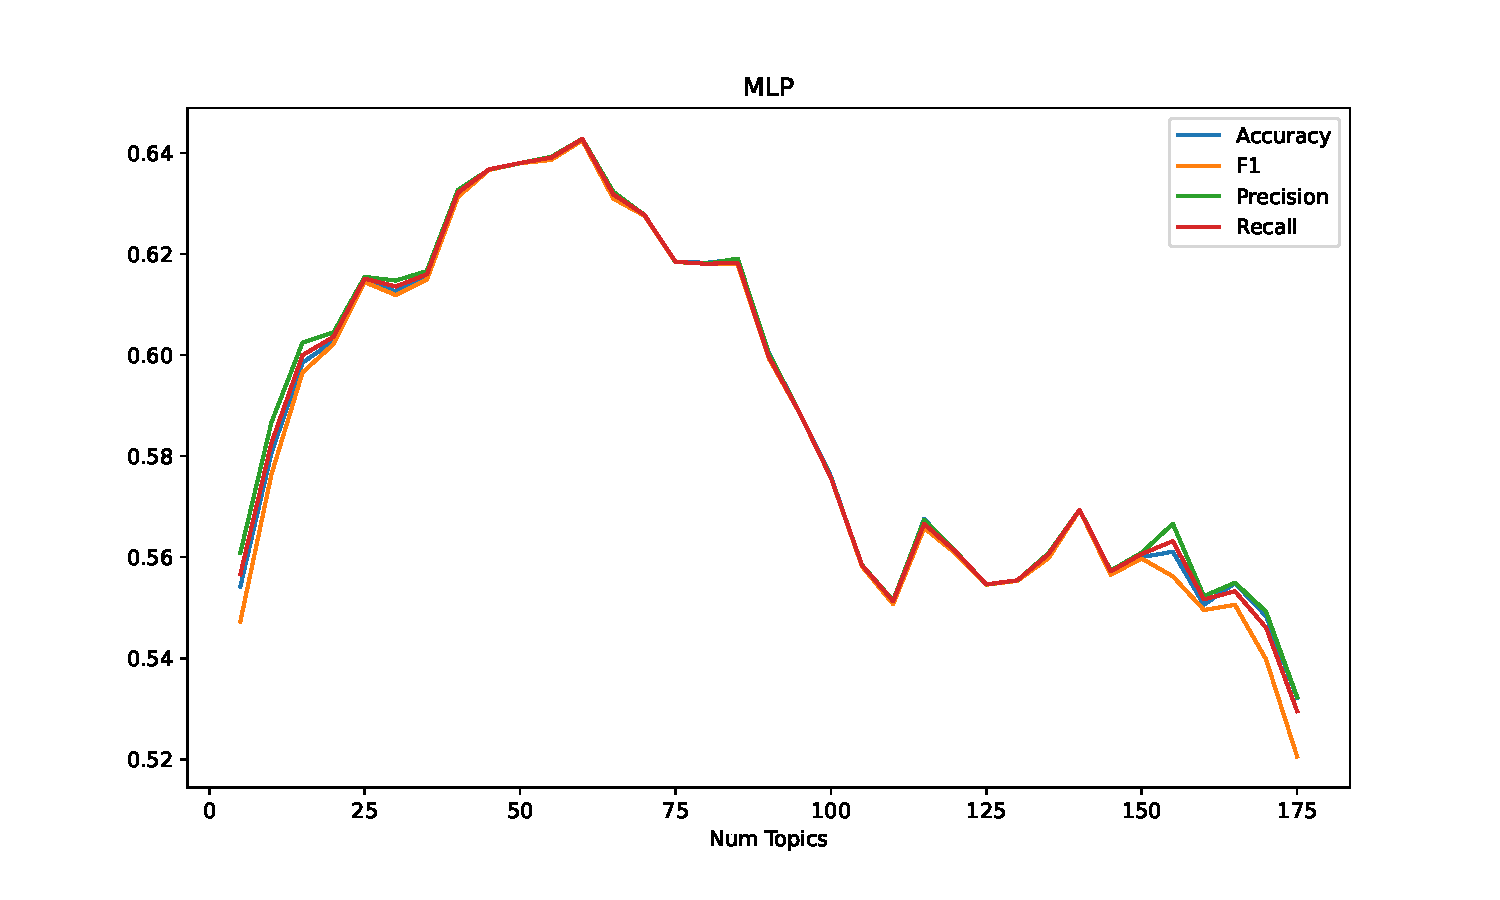
\includegraphics[width=\linewidth, trim={2cm 0.7cm 2cm 1.6cm}, clip]{figures/40k/evaluation_mlp.pdf}
	\caption{Performance of MLP}
	\label{fig:p_mlp}
\end{figure}

\begin{figure}[h]
	\centering
	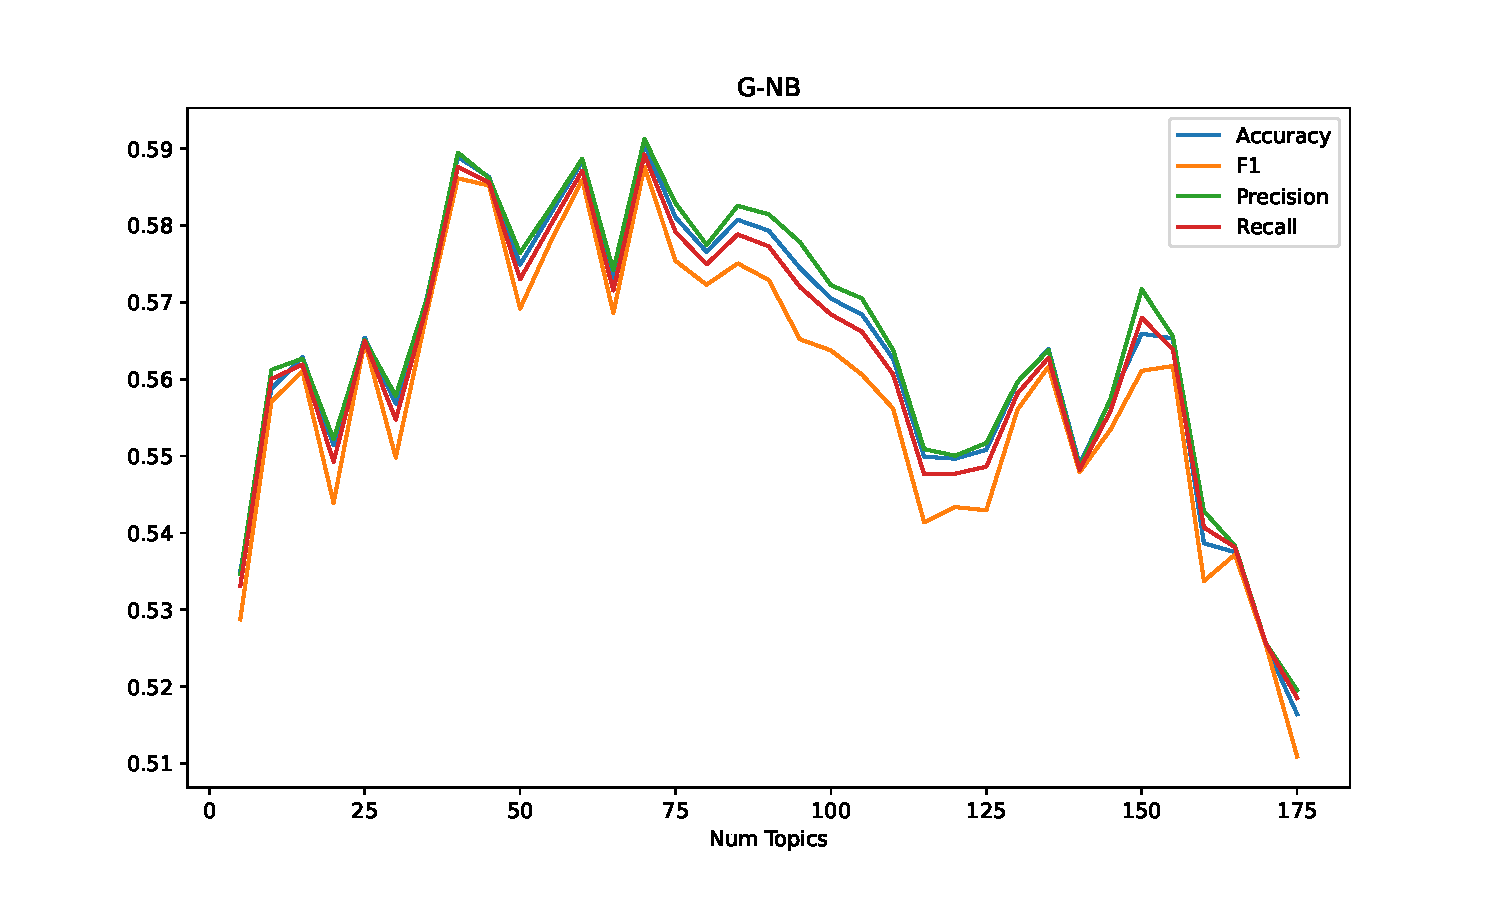
\includegraphics[width=\linewidth, trim={2cm 0.7cm 2cm 1.6cm}, clip]{figures/40k/evaluation_g-nb.pdf}
	\caption{Performance of G-NB}
	\label{fig:p_gnb}
\end{figure}

\begin{figure}[h]
	\centering
	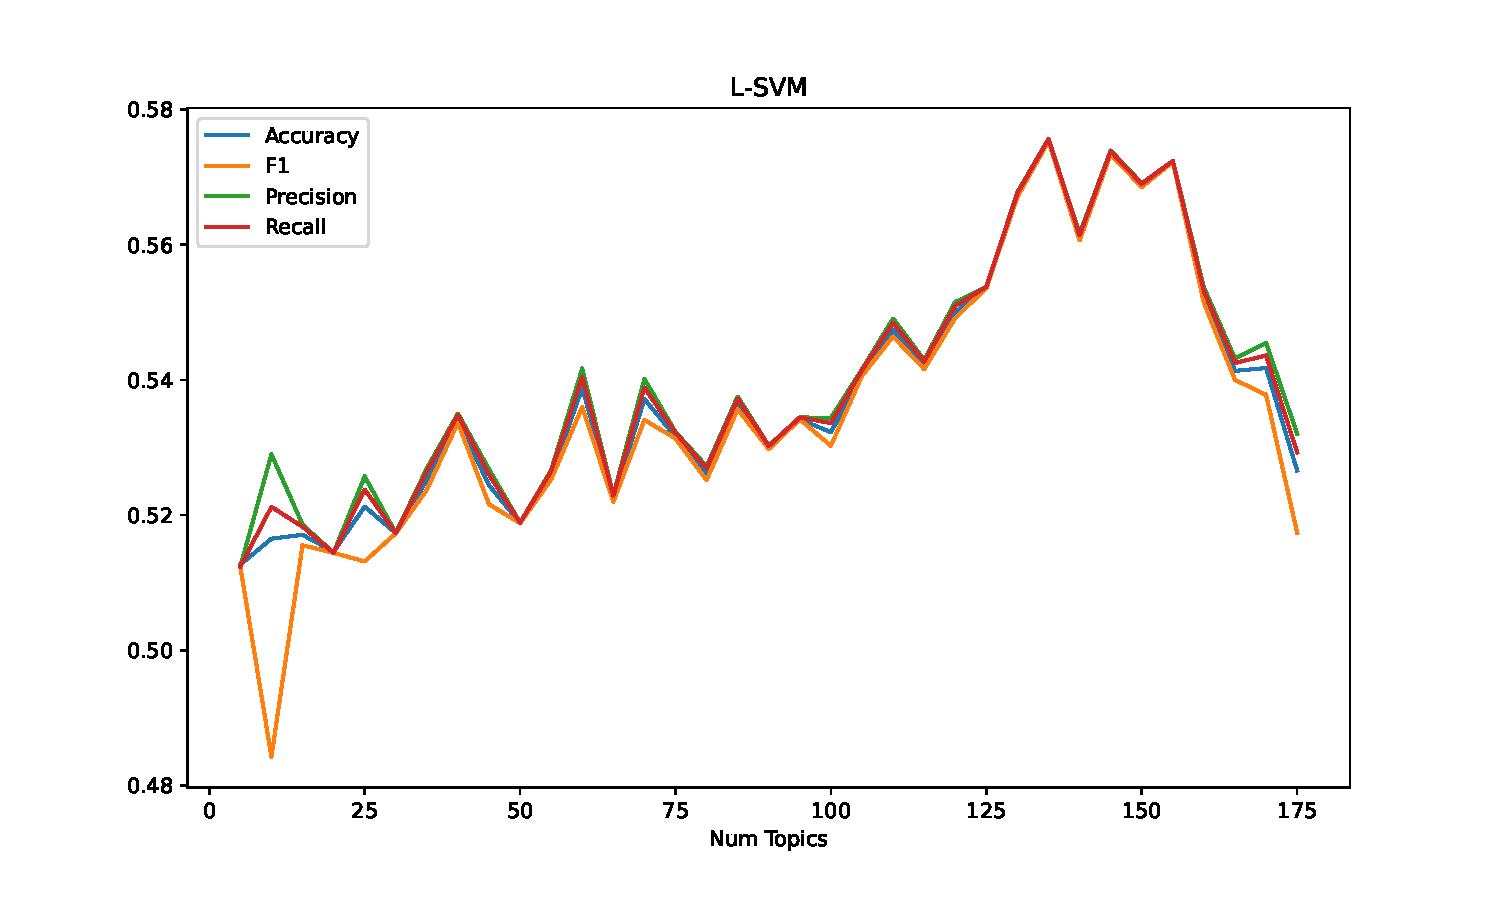
\includegraphics[width=\linewidth, trim={2cm 0.7cm 2cm 1.6cm}, clip]{figures/40k/evaluation_l-svm.pdf}
	\caption{Performance of L-SVM}
	\label{fig:p_lsvm}
\end{figure}

In the range from $k=5$ to $k=100$, we can see a clear advantage of the MLP over the other classifiers. The MLP classifier also has the overall highest accuracy at $k=60$.
A similar behavior but with an overall lower score can be seen for the G-NB. 
The L-SVM is showing the worst performance rising from the start with a peak at $k=130-150$ where a rapid drop of perplexity was observed previously.

During the comparison, all classifiers were trained with their default parameter settings. 
After determining MLP as the best performing classifier, hyperparameter optimization was performed using grid search.

\begin{figure}[h]
	\centering
	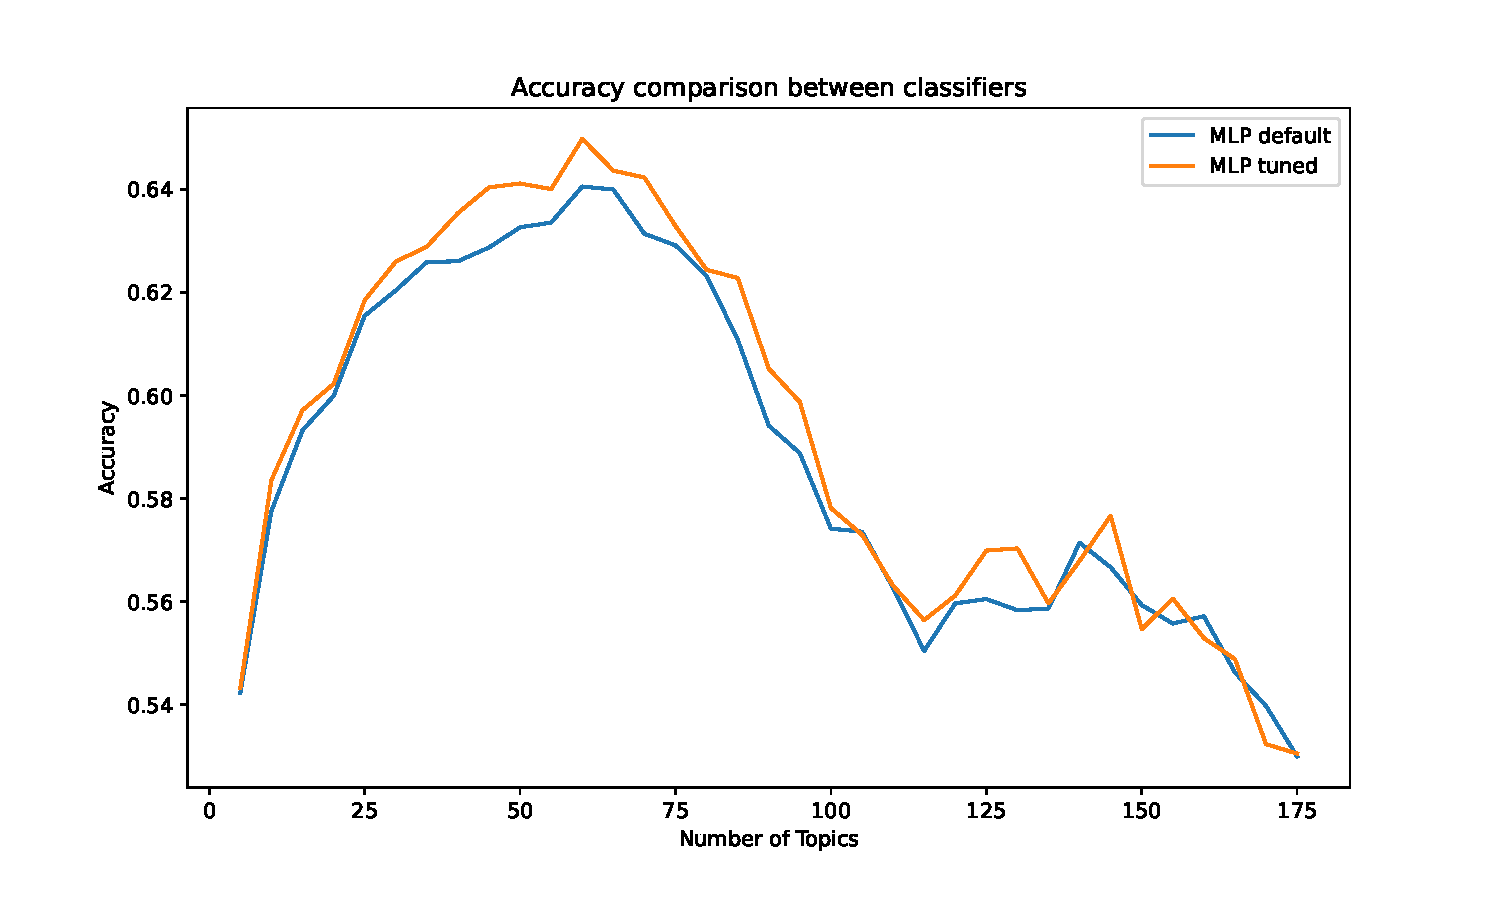
\includegraphics[width=\linewidth, trim={2cm 0.7cm 2cm 1.7cm}, clip]{figures/MLP_default_vs_tuned/classifier_accuracies_over_topics.pdf}
	\caption{MLP accuracy default and tuned parameters}
	\label{fig:mlp_default_tuned}
\end{figure}

Figure \ref{fig:mlp_default_tuned} shows a comparison between a MLP classifier with default parameters and the tuned parameters from the grid search. 
With the tuned parameters an overall improvement can be observed.
As before with default parameters the highest accuracy can be seen at $k=60$.

A further factor with a big impact on the performance of all classifiers is the amount of tweets used.

\begin{figure}[h]
	\centering
	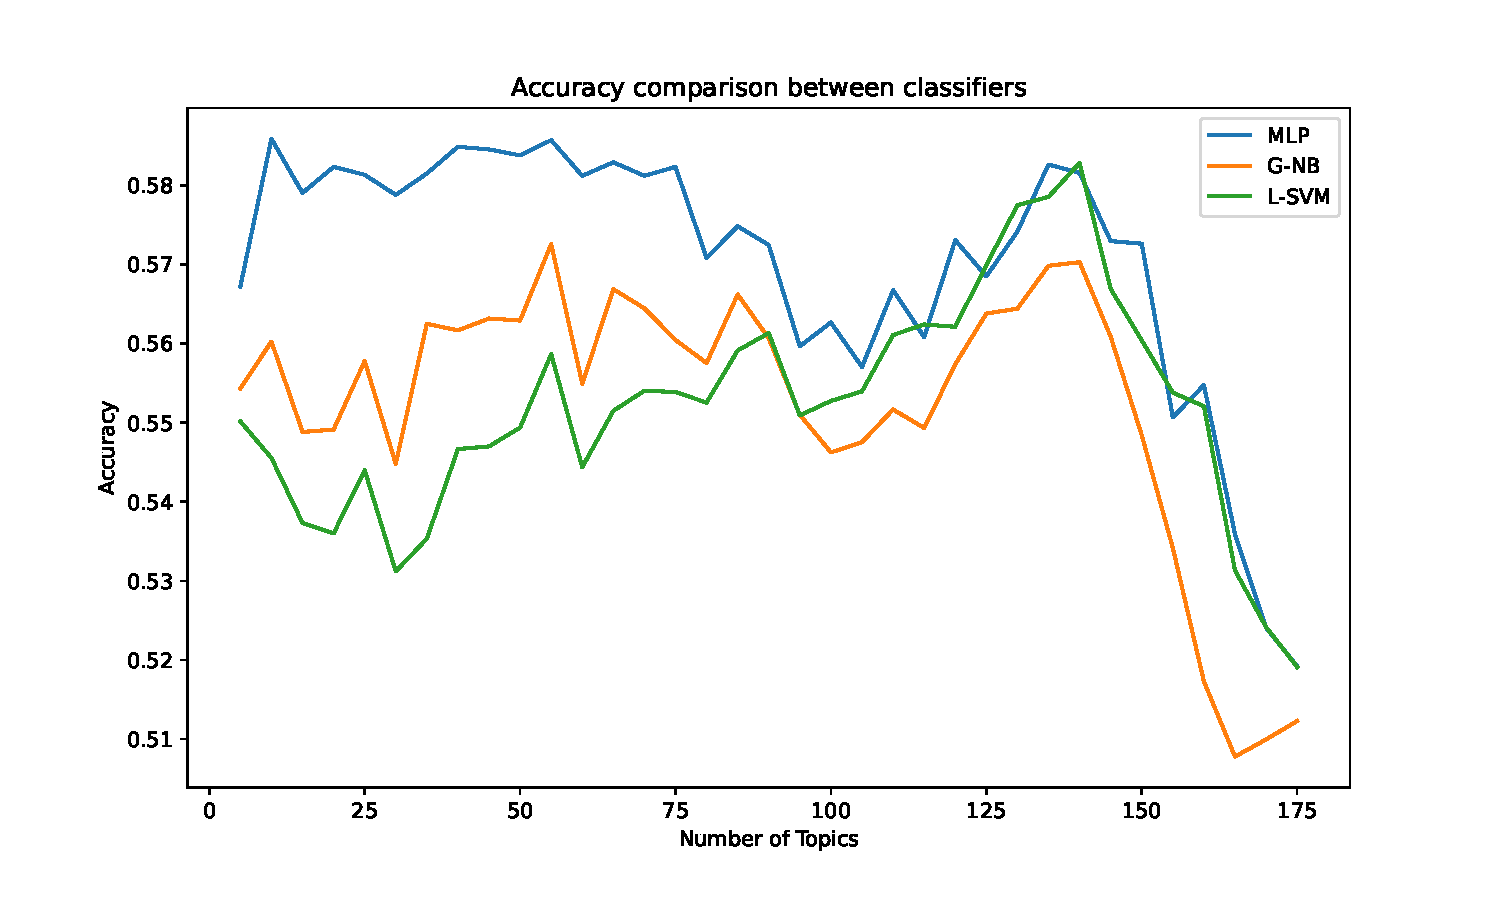
\includegraphics[width=\linewidth, trim={2cm 0.7cm 2cm 1.7cm}, clip]{figures/80k/classifier_accuracies_over_topics.pdf}
	\caption{Accuracy with 80,000 tweets}
	\label{fig:acc_80k}
\end{figure}

For the previous performance measurements 40,000 tweets were used, with an even distribution between members of the Democratic or Republican Party. 
In figure \ref{fig:acc_80k} an overall lower accuracy for all classifiers is shown using 80,000 tweets. 

\begin{figure*}[ht]
	\centering
	\begin{subfigure}[b]{0.45\textwidth}
		\centering
		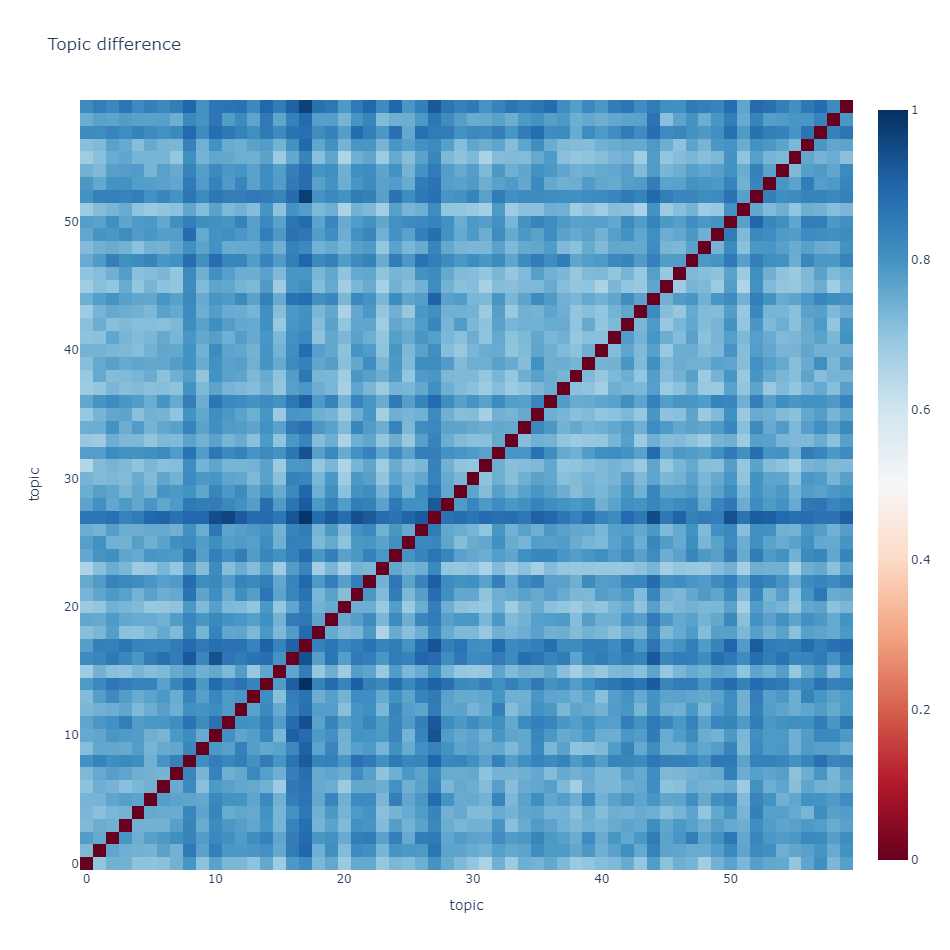
\includegraphics[width=\textwidth, trim={1cm 1cm 1cm 2cm}, clip]{figures/40k/diff_matrix_plotly.png}
		\caption{40,000 tweets}
		\label{fig:diff_mtx_40k}
	\end{subfigure}
	\hfill
	\begin{subfigure}[b]{0.45\textwidth}
		\centering
		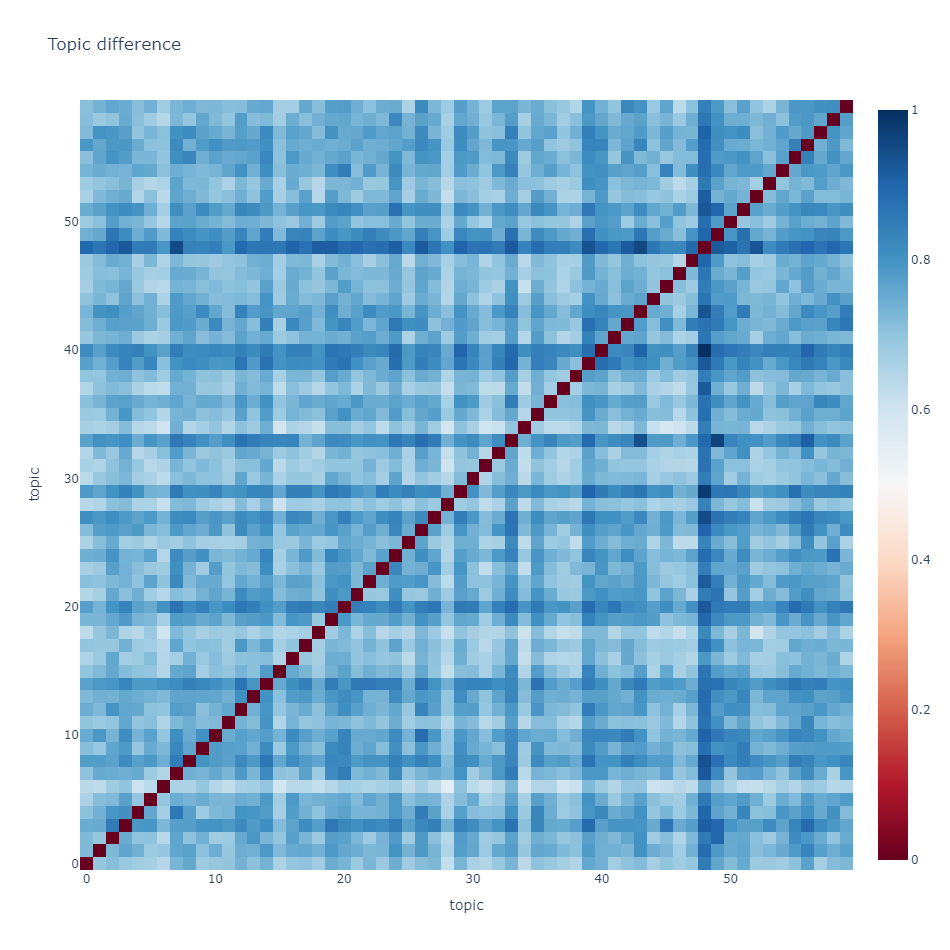
\includegraphics[width=\textwidth, trim={1cm 1cm 1cm 2cm}, clip]{figures/80k/diff_matrix_plotly.png}
		\caption{80,000 tweets}
		\label{fig:diff_mtx_80k}
	\end{subfigure}
	\caption{Pairwise dissimilarity of 60 topics created with differing number of tweets}
	\label{fig:topic-dissim}
\end{figure*}

The drop in accuracy with increased tweets can be explained with a lower dissimilarity between topics. 
Figure \ref{fig:topic-dissim} is showing a comparison between two dissimilarity matrices from LDAs with 60 topics using 40,000 and 80,000 tweets. 
The overall lighter blue of the matrix in \ref{fig:diff_mtx_80k} indicates a lower distinction between topics. 
Therefore vector embeddings becoming more homogeneous, resulting in lower performance of the used classifiers.

In conclusion, the best performance was found with 40,000 tweets using MLP classifier with tuned parameters achieving an accuracy of 0.651.

The shown approach presumes the same LDA is used for embedding the training and test data. 
When splitting the data and creating separate LDAs for test and training, the accuracy drops to 0.50 using the MLP classifier.

\section{Summary}
\label{sec:summ}
To summarise the findings of this approach it is clear, that using LDA as embedding for classifiers does not produce sufficient results. 
Even in this best-case scenario having only two parties and tweets from politicians rather than citizens it was not possible to obtain reliable predictions of the author's political view.

Therefore, it seems that unsupervised, generative LDAs are unable to capture semantic meaning towards certain, for the political position relevant topics, by using statistical methods.

Further work could investigate, whether supervised methods, especially Deep Learning, bare better solutions to this task. 
For example one may fine tune existing and overall well performing transformer models such as BERT for this classification task.

%\clearpage
\bibliographystyle{ACM-Reference-Format}
\bibliography{sample}
\end{document}
\endinput
